\documentclass[brazil, bsc, 10pt]{beamer}
%\usetheme{default}
\usecolortheme{dove}
\usepackage[utf8]{inputenc}
\usepackage{lastpage}		
\usepackage{indentfirst}
\usepackage[alf]{abntex2cite}	
\usepackage{tikz}
\usepackage{circuitikz}
\usepackage{graphicx}
\usetikzlibrary{arrows.meta, positioning, shapes, fit}
\usepackage{lipsum}
\usepackage[english]{babel}
\usepackage[linesnumbered]{algorithm2e}
\setbeamertemplate{navigation symbols}{}
\usepackage{listings}
\usepackage{minted}

\tikzstyle{box} = [rectangle, rounded corners, minimum width=3cm, minimum height=1cm, text centered, draw=black, fill=gray!20]
\tikzstyle{arrow} = [thick, ->, >=stealth]

\title[Intro]{I/O Patterns and Bottlenecks in Deep Learning Workloads}
\author[Hugen]{
  Pablo Alessandro Hugen\inst{1}
}

\institute[UFRGS]{
  \inst{1}%
  Institute of Informatics -- UFRGS\\
}

\date[2024]{
  Comp. Sys. Perf. Analysis 2025/2
}

\logo{%
  \makebox[0.95\paperwidth]{%
      \includegraphics[width=2cm,keepaspectratio]{images/logo-ufrgs.png}
    \hfill%
    \includegraphics[width=2cm,keepaspectratio]{images/logo-ppgc.png}
  }%
}
\AtBeginSection[] {
  \begin{frame}<beamer>{Content}
    \tableofcontents[currentsection]
  \end{frame}
}

\begin{document}

\frame{\titlepage}
\logo{}

\section{Introduction}

\subsection{Context}

\begin{frame}
	\frametitle{Context}

	\begin{block}{}
		\begin{itemize}
			\item Recent growing interest in optimizations for Machine Learning/Deep Learning
			      training and inference methods.
			\item Used in various fields: LLMs, Image reconition and classifications, and so on.
			\item Large models often need very large HPC infraestructures for
			      processing the insane amount of training data.
			\item The performance of the storage and I/O subsystem of HPC systems is critical

		\end{itemize}
	\end{block}
\end{frame}

\begin{frame}
	\frametitle{Context}

	\begin{block}{}
		\begin{itemize}
			\item Traditional HPC workloads are characterized by large, sequential data access \cite{characterizing_ml_io_workloads}.
			      \begin{itemize}
				      \item Simulations which saves the state at the end or in checkpoints
			      \end{itemize}

			\item In contrast, ML workloads generate small, random reads across numerous files \cite{characterizing_ml_io_workloads}.

			\item Large amounts of data (far greater than system memory) + random read pattern = lot of page faults and cache misses (VERY BAD)
		\end{itemize}
	\end{block}
\end{frame}

\begin{frame}
	\frametitle{Context}
	\begin{center}
		\includegraphics[width=0.8\textwidth]{./images/latencies.png}
	\end{center}
\end{frame}

\begin{frame}
	\frametitle{Context}

	\begin{block}{}
		\begin{itemize}
			\item At Large Scale Distributed DL Workloads, IO can take roughly 85\% of the \emph{training} time \cite{clairvoyant_prefetching_for_distributed_ml_io}.
			\item And training is often one of the most expensive parts of the pipeline \cite{io_machine_learning_applications}.
		\end{itemize}
	\end{block}
	\begin{center}
		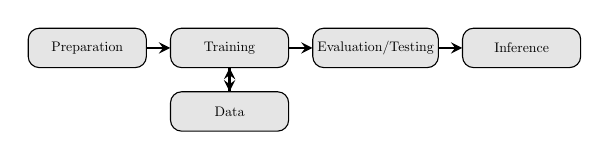
\begin{tikzpicture}[
				node distance=0.6cm,
				auto,
				scale=0.5,
				transform shape
			]

			\node[box] (prep) {Preparation};
			\node[box, right=of prep] (train) {Training};
			\node[box, right=of train] (eval) {Evaluation/Testing};
			\node[box, right=of eval] (infer) {Inference};

			% New "Data" node below Training
			\node[box, below=of train] (data) {Data};

			\draw[arrow] (prep) -- (train);
			\draw[arrow] (train) -- (eval);
			\draw[arrow] (eval) -- (infer);

			% Arrows between Training and Data
			% One arrow from Training to Data
			\draw[arrow] (train.south) -- (data.north);
			% One arrow from Data to Training
			\draw[arrow] (data.north) -- (train.south);

			% Alternatively, a single bidirectional arrow:
			% \draw[bidirectional_arrow] (train) -- (data); 
		\end{tikzpicture}
	\end{center}
\end{frame}


\subsection{Objectives}

\begin{frame}
	\frametitle{Objectives}
	\begin{block}{General:}
        Understand \alert{patterns in I/O operations and possible bottlenecks} in common
        Machine Learning workloads
	\end{block}
	\begin{block}{Específicos:}
		\begin{itemize}
			\item \textbf{Revisão bibliográfica}: Base teórica para o desenvolvimento do simulador.
			\item \textbf{Implementação do Simulador}: Aplicar os conceitos de paralelismo assíncrono e hetereogêneo em CPUs e GPUs.
			\item \textbf{Validação do simulador}: Ratificar \alert{aspectos computacionais e de desempenho} da implementação.
		\end{itemize}
	\end{block}
\end{frame}

\subsection{Related Works}

\begin{frame}
	\frametitle{Trabalhos Relacionados}
	\begin{block}{\citeonline{aaby2010efficient}}
		Focou na otimição de um simulador multiagente utilizando CUDA em multi-GPU, com comunicação MPI e foco em reduzir a latência. Resultados mostraram uma performance 100 vezes maior.
	\end{block}

	\begin{block}{\citeonline{shekh2015hybrid}}
		Portaram simuladores multiagente para multi-GPU e analisaram a escalabilidade. Resultados mostraram eficiência com populacoes de até 100 milhões de agentes.
	\end{block}
\end{frame}

\begin{frame}
	\frametitle{Trabalhos Relacionados}
	\begin{block}{\citeonline{cunha2022aperfeiccoamento}}
		Focou na otimização paramétrica do modelo de espalhamento de dengue, obtendo resultados satisfatórios.
	\end{block}

	\begin{block}{\citeonline{lin2022evaluating}}
		Mostrou a viabilidade da utilização do padrão \textit{Iso C++ 17 Parallel STL} em GPUs para a otimização de algoritmos paralelos em comparação com OpenMP, CUDA e o SYCL. Mostrou uma performance equivalente, com excessão de alguns casos específicos.
	\end{block}

	\begin{block}{\citeonline{gomez2023gpu}}
		Implementou um solucionador de sistemas de equações diferenciais parciais em GPUs utilizando o padrão \textit{Iso C++ 17 Parallel STL} e o SDK da NVIDIA. Porém,resultou em uma performance inferior em comparação com o OpenMP.
	\end{block}
\end{frame}


\begin{frame}[allowframebreaks]
	\frametitle{Bibliography}
	\bibliography{references}
\end{frame}

\end{document}
